\chapter{Introduction}
\label{cha:intro}

In this chapter we begin by outlining the justifications behind our research into this field, highlighting the absence of current work accounting for stochastic routing in the field of network tomography in \cref{sec:Imotivationandoutline}. We then identify specific sub-problems within the existing work on stochastic routing and pose solutions to these problems in the form of project wide scope goals. Next an overview of current models and inferential techniques used in stochastic network tomography is provided in \cref{ssec:Icurrentmodels} through decomposition of these models into their three major components: network generation, traffic simulation and inferential calculations. We then present new metrics used within our tomographic method, namely packet delay variation and the related notion of alternative fixed probe routing methods. These new approaches for stochastic tomography are compared and contrasted to current methods, with focus on trade-offs between nefarious classification confidence, method time/space complexities and model robustness in \cref{sec:Iinferentialtechniques}. Lastly we establish mathematical approaches used to give concrete bounds to the accuracy of our inferential classification of nefarious nodes and give an overview of approaches to inverse problems and optimality in \cref{sec:Icoreconcepts}.\par

\newpage
\section{Motivation and Outline}
\label{sec:Imotivationandoutline}

Network Tomography is the technique of using end-to-end measures to make inferences about that computer network. In this way it is similar to computed axial tomography (CAT) scans in the medical world where x-rays are passed through a patient as a noninvasive method of gaining information pertaining to the interior of the patient. These x-rays are fired from multiple points around the exterior of the patient, they attenuate as they pass through different densities of the tissue and are measured as they exit the body. This process results in a single 2 dimension ‘slice’ of tissue density in the body being calculated. This is typically repeated over many slices next to one another to give a 3 -dimensional representation.\par
Network tomography is most analogous to a single one of these slices however instead of using the attenuation of x-rays to infer body tissue density we observe the latency of communication to infer the structure and behaviour of routers within a network, a high level illustration of the problem is given in \ref{fig:nettom?}. In network science this latency is referred to as a delay and is calculated from the time a given ‘packet’ or discrete signal takes to traverse the network to its predetermined destination. It should be noted that although in network science there are various forms of signal casting - primarily broadcasting, uni-casting, multi-casting, and any-casting - we will focus on the case of a uni-casted signal. This is as the inclusion of alternative casting methods introduces enough complexity to the analysis that tomography under each casting method has spawned its own sub field of research (\cite{lawrence_network_2006}).\par
\begin{figure}
    \centering
    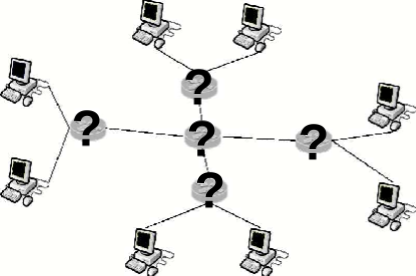
\includegraphics[width=10cm]{figs/intro/nettom-illustration.png}
    \caption[Illustrative example of network requiring tomographic probing]{Illustrative example of network requiring tomographic probing \cite{lawrence_network_2006}}
    \label{fig:nettom?}
\end{figure}

The primary motivations for network tomography are topology identification (\cite{zhang_topology_2014}, \cite{hailiang_network_2009}), general internal state inference (\cite{vardi_network_1996}, \cite{coates_network_2001}, \cite{he_network_2021}) and in the case of Boolean tomography, node failure localisation (\cite{nguyen_boolean_2007}, \cite{ma_optimal_2015}). In this body of work we focus on internal state inference, specifically in the form of identification of abnormal behaviour of network components, potentially caused by a nefarious actor intent on disrupting network behaviour. As such we refer to these induced cases of abnormal behaviour and the offending network components causing these as ‘nefarious’. We take this lens as the existence of adversarial settings is a key differentiator between theoretical and real world applications of any technology.\par
As network tomography is maturing it is beginning to be implemented in many real world settings with support from emerging protocols and platforms such as Consul \cite{shilton_network_2021} and future support in the form of network coding based approaches discussed in \cite{kakkavas_review_2020}. The increasing use of this in real world settings therefore demands research into methods of further validating and optimising the performance of network tomography in these industrial, public and private  communication infrastructure settings.\par
Historical work on uni-cast tomography focuses primarily on networks with an absence of queue buffers, resulting in packet’s taking static paths through a network. This assumption was relaxed by \cite{lai_measuring_2000} in their work focusing on routing behaviours resulting in stochastic routing networks. Recent work by \cite{barnes_stochastic_2020} has used this approach to introduce nefarious behavior in stochastic settings and subsequently detect this behaviour. In doing this the simulation developed was made more applicable to real world networks.\par
We aim to build upon this work of nefarious behaviour detection in stochastic environments by relaxing further assumptions in order to better simulate mid-sized complex real world networks such as a home or IoT network. We focus on ensuring methods employed are scalable to far larger networks in hope of maintaining general applicability to large scale real world networking such as that in academic, consumer ISP and commercial data center networks underlying modern cloud infrastructure. The key assumptions under which Barnes based their work are:\par
\begin{enumerate}
\item \emph{End Nodes of the network are switches.}
\item \emph{All packets originate and terminate at switches.}
\item \emph{All routers which are not nefarious behave identically.}
\item \emph{Packets are not dropped when traffic is heavy, instead accumulating in queues of unbound length.}
\item \emph{Background traffic across the network has a constant average intensity.}
\item \emph{All end nodes are equally likely to send packets, and be chosen to receive packets.}
\item \emph{All routing protocols are the same for non-nefarious routers.}
\item \emph{The service time for every packet at the front of the queue in a router is 1 “Time step”.}
\end{enumerate}

We focus on the relaxation of 2, 3, 4, 6, 5 and 7 and leave future work to address additional simplifications. These were chosen as assumption 1 allows for a bounded network size as without switches as end nodes we would be forced to instead model all sub-networks which are connected to these switches, and the networks connected to the switches of those sub-networks recursively. This would eventual end in the model representing the observable internet connected to this network, thus being unbounded in size and therefore both impractical and non useful to analyse. We instead maintain this assumption to allow for analysis of arbitrary sub-networks which may be of interest to the typical network administrator, with adjacent networks able to represented a single node with a number of switches connected proportionally to the typical traffic from that network. Assumption 8 is key to the analysis technique used within our work, the difficulty behind its relaxation is expanded in \cref{sec:Rnefarouterdetection}, but the relaxation of this particular assumption is left to further work on the topic.\par
In the implementation of these complex behaviours resulting from this relaxation we hope to accomplish a primary goal of ensuring the established mechanisms for gaining tomographic inference are robust enough to identify nefarious behaviour in complex real-world systems. Given the complexity of real world implementation pales in comparison to that of previous mathematical models we introduce alternative methods of tomography, namely \pdv tomography in \cref{sec:Iinferentialtechniques} with the purpose of utilising it to overcome these hurdles of complexity.\par
Although this results in less accurate classification of nefarious nodes, we utilise optimization techniques presented in \cref{sec:Boptimization} and \cref{ssec:Bparsppselection} to maximise the inferential accuracy of our new methods. For the purpose of quantifying both the observed and maximum potential accuracy of our inference we adapt statistical methods from link focused tomographic studies in \cite{he_fisher_2015}. In doing this we represent all information known about the given network using the notion of Fisher information explained in \cref{ssec:Bfisherinformation}, allowing for computation of the maximal inferential power in the form of the Cramér–Rao Bound subsequently covered in \cref{ssec:Bcrb}\par
Finally we aim to use this exploration to complete two secondary objectives relating to network tomographic inference of nefarious nodes within a network. Firstly to fix inconclusive results in the work of Barnes relating to the impact of monitor placement algorithms on identifiability of nefarious router sets. Secondly, in the vein of \cite{zhao_measurement_2020}, we lay the framework for the inclusion of alternate attack methods into complex stochastic tomographic models and quantify the effect of these attacks on the power of tomographic inference. The importance of the analysis of tomography accuracy in such adversarial settings is still a fledgling field of research with very few studies on the topic as noted in a compilation of current work in \cite{he_network_2021}.

\newpage

\section{Stochastic Network Tomographic Models}
\label{sec:Imodels}

In this section we introduce existing models and methods for stochastic network tomography in literature, for ease of discussion and to aid reader digestion we split these models into three sections: network generation, traffic simulation and inferential calculations. This decomposition was chosen as each section can be treated as a distinct process, with the output from each able to be parsed to the next in a context-free manner. Within \cref{ssec:Icurrentmodels} we cover specific methods currently used for each of these three areas with a primary focus on the traffic and delay simulation in \cref{sssec:Itrafficsimulation}, highlighting assumptions and key segments for potential improvement. Finally we provide an overview of the model produced as a key deliverable of this project, outlining differences from the current work.

\subsection{Preexisting Models}
\label{ssec:Icurrentmodels}

Current work surrounding network tomographic models identifying nefarious nodes in stochastic networks is led by the work of \cite{barnes_stochastic_2020}. This work falls under the previously mentioned mathematicians approach to tomography and was based upon the requirement that the system must be formally mathematically modelable. Over this section we introduce approaches used in this work along with candidate areas considered for extension with the intent of providing additional explanation and background of these techniques in \cref{cha:background}. We note that work within both \cite{he_fisher_2015} and \cite{kolar_distributed_2020} also covers stochastic environments however both studies focus on link level metrics. However in \cref{ssec:Idevelopedmodels} we show how techniques within work on link metrics can be adapted for use within our work.

\subsubsection*{Network Generation}
\label{sssec:Inetworkgeneration}

The goal of network generation in the context of validating tomographic models is production of a random undirected graph representing a small to medium sized network. The generated network must contain 4 essential components, routers to direct packets, links between routers for packets to traverse, Switches which emulate connection to a larger external network (i.e. the world wide web) through stochastic production of packets (elaborated upon in \cref{sssec:Itrafficsimulation}) and Monitors, particular switches in tomographic analysis which we are able to directly control and observe. Each of these components is represented as a node within the graph. The generation of these pseudo random networks is desirable for verification of tomographic techniques in a controlled environment as it allows for many topologies to be tested to ensure robustness of introduced techniques.\par
Current work around nefarious router identification in stochastic networks by \cite{barnes_stochastic_2020} uses a user defined connectivity parameter to generate edges between nodes. This is analogous to the Erdos-Renyi (ER) generation technique originally posed in \cite{erdos_random_1959}, we provide formal definitions of this technique in \cref{sec:Bgraphgeneration}. In real world networks however, router degree (number of connected routers and switches) converges to a power law i.e. the distribution of router degree in a sufficiently large network as shown in \ref{fig:nddist} (\cite{chen_origin_2002}, \cite{zhao_measurement_2020}) - such graphs are commonly referred to as “scale-free”. In contrast to this, a Poisson distribution of node degree is observed in other more naive network generation algorithms such as the Erdős–Rényi model as shown compared to scale free graph \ref{fig:nddist}.
\begin{figure}[ht]
    \centering
    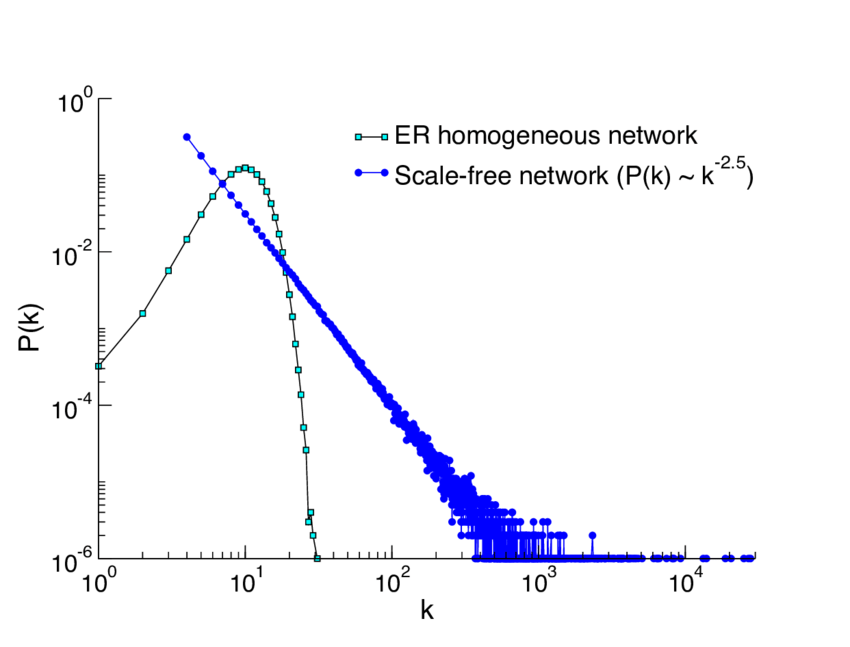
\includegraphics[width=10cm]{figs/intro/nodedegree-dist.png}
    \caption[Distribution of node degree in a generated network]{Distribution of node degree in a generated network (note log scale of the x-axis) \cite{baronchelli_networks_2013}}
    \label{fig:nddist}
\end{figure}
Existing work on stochastic network tomography primarily from \cite{thoppe_stochastic_2014} \cite{kolar_distributed_2020} represents networks in a tree based topology. As noted in \cref{cha:litreview} This technique is common practise when utilizing multi cast packet transmission for inferential calculations. Such tree based models, although useful for simplifying tomographic problems, are poor representations of real systems, we expand further on the discrepancies in \cref{sec:Bgraphgeneration}.

\subsubsection*{Traffic Simulation}
\label{sssec:Itrafficsimulation}

The accumulation of all packets sent between each node in the network (referred to as network traffic or simply traffic) and it’s simulation is a key aspect of any network model. Intuitively the traffic within a network is an accumulation of all packets sent from each switch within that network.The traffic at any single router is therefore determined by the number of components adjacent to it, and their respective routing tables, and number of packets they are forwarded. The current model used within the work of \cite{barnes_stochastic_2020} splits traffic simulation into discrete time steps of a uniform length, we adopt their assumption that each time step is a period small enough that only a single packet is handled by each router in each step and expand on this in \cref{ssec:Idevelopedmodels}. \par
Due to this discretization of network traffic, packets (as one would anticipate) do not traverse from sender to receiver instantly, but rather are delayed throughout their path. We adopt terminology from the authoritative work of \cite{kurose_computer_2013} and decompose this delay into four classes: processing, transmission, propagation, and queuing delays. Processing delay is the time required for a network component to analyse the requirements of a packet and action on those requirements. Transmission delay is simply the time taken for the link interface of a network component to push the physical bits representing the information onto the transmission interface (i.e. fibre, copper, wireless...). Propagation delay is the time taken for the signal to traverse the transmission interface from sender to receiver, largely dependent on the type of medium and physical distance between components. Lastly, queuing delay for the purposes of our work is defined as the delay a packet experiences waiting in the buffer of a router, and has begun to be explored explicitly in previous work.\par
As multiple packets in existing models may be forwarded to a single router each time step and each router is only able to perform one forward a time step these packets can accumulate in the respective routers’ queues, awaiting forwarding. These router queue lengths are therefore analogous to queuing delays in real world systems. The work of \cite{barnes_stochastic_2020} considers only the class of queuing delays when dealing with packet delay measurements, where other work on stochastic tomography \cite{kolar_distributed_2020}, \cite{he_fisher_2015} makes no distinction between delay classes, instead dealing only with the generalised concept. As noted in \cite{telchemy_impact_2006} in realistic applications, propagation and processing delays are negligible, we therefore focus on primarily extending the work of \cite{barnes_stochastic_2020} and their focus on queuing delays.\par
In addition to this we explore impacts of the cumulation of all delay classes on our model via implementation in real network simulators within \cref{sec:Rrealnetworkperformance}. Although all packets in a network experience these delays, the magnitude of the delays is ultimately dependent on the number of packets within the system at any given point in time, or as it is commonly referred to, the traffic intensity.\par
Traffic intensity is a result of the number of packet sent over a network by nodes, generation of such network traffic has been shown to be binomial distribution (\cite{barnes_stochastic_2020}) over a set time window which approaches a Poisson distribution over a large enough number of time steps. From (\cite{barnes_stochastic_2020}), where $n$ denotes the number of time steps, $k$ being the number of packets sent and $s$ being the probability on any given time step that a packet will be sent:
\[\lim_{n\to\infty} \frac{n!}{k!(n-k)!}s^k (1-s)^{n-k} =\frac{s^k e^{-s}}{k!}\]
This known distribution of traffic intensity is key in the current body of work as it allows for the traffic being sent from a node to be represented as a random variable S with a known distribution and a value of 1 or 0 depending on if a packet is sent or not. \par
Similarly to that of packets, queue lengths and consequently queuing delay can be expressed as a random variable \gls{qlen}. Prior work assuming constant average traffic intensity has shown that \gls{qlen} both converges to a steady state over time and, given its dependency on the queue length at the previous time step, is a Markov process (\cite{barnes_stochastic_2020}). However, \gls{qlen} for each router is a consequence of not only the number of packets sent $S$, but also the paths these packets take through the network; the routing method used by the network therefore must be scrutinised to utilize a Markov chain model to quantify \gls{qlen} as shown in \cite{barnes_stochastic_2020}.\par
For network traffic to be complexly stochastic any routing protocol must be dynamic in nature, else fixed routing tables would be established and only a single path would be taken by a packet between any two nodes within the network resulting in the only traffic variance coming from packet generation rate of switches. Current work uses an abstract implementation of the distance vector routing protocol (\cite{perkins_ad_2003}) to achieve this dynamic routing behaviour, with a global controller using Dijkstra's algorithm to compute the shortest distance between any two given nodes and broadcast this information to all components in the network (\cite{barnes_stochastic_2020}). In this method edge weights for the computation are representative of the number of packets waiting in the queues of each router at the end of that edge as this is analogous to the number of time steps a packet would wait before completing it’s traversal of that edge.\par
The use of a network wide controller in this manner is akin to that of Software Defined Networks (SDNs) where routing logic at the link level is dynamically handled by an SDN controller - we refer the keen reader to the excellent survey by \cite{kreutz_software-defined_2015} for additional information. As most commercial grade networks do not employ SDNs currently and the security concerns surrounding widespread adoption of SDN to control for all  traffic on a network moving into the future (\cite{wood_scalable_2021}) we highlight the decentralization of this background traffic routing as a key area of work addressed in \cref{sec:Broutingmechanisms}.\par
In the work of \cite{barnes_stochastic_2020} no distinction is made at a routing level between different types of traffic that the router is forwarding, a packet sent by a monitor node that we are able to draw inference from is treated identically to all other packets. As in \cref{sec:Mnetworkprobing} we adopt the terminology of \cite{he_network_2021} and refer to this as uncontrolled routing (UR), where packets which we are able to observe, as they are sent between monitor nodes, follow the underlying routing behaviour of the network. As routers are able to make distinctions between packets and forward them accordingly, distinction and alternate routing of probe packets from monitors is feasible under both normal and SDN conditions. Due to our model varying only the routing restriction for these probe packets from monitors, we use the term routing to refer exclusively to these cases, addressing other traffic as background traffic when required. We introduce the alternative forms of routing originally presented in \cite{he_network_2021} and outlined in further detail in \cref{sec:Broutingmechanisms}, as key targets for extension of the existing model.

\subsubsection*{Inferential Calculations}
\label{sssec:Iinferentialcalculations}

Current work in \cite{barnes_stochastic_2020} utilizes a combined agent based and Markov Chain Monte Carlo (MCMC) approach for approximating the expected delay given a subset of routers are nefarious. This method allows for extremely accurate calculation of nefarious nodes compared to conventional methods of link inference tomography but has significant time and space complexities. The computation of expected delay distributions for each subset of nefarious routers intuitively takes on the order of number of router combinations $\mathcal{O}(2^{|R|})$. Previous work in \cite{belloni_computational_2009} has established the complexity of an MCMC algorithm over a large sample space as $\mathcal{O}(d^3 log d)$ where d is the dimensionality of the sample space, or network in our case, which is known to be $\leq 2\cdot \gls{maxdeg} N + 1$ (\cite{erdos_chromatic_1980}). The total complexity of this method is therefore on the order of:
\begin{align}
\label{eq:mcmcbigo}
    \begin{split}
        &\mathcal{O}( (2\cdot \gls{maxdeg} N + 1)^3 \cdot log(2\cdot \gls{maxdeg} N + 1)\cdot 2^{|R|})\\
        &\mathcal{O}(\gls{maxdeg} N ^3 \cdot log \gls{maxdeg} N \cdot 2^{|R|})
    \end{split}
\end{align} we aim to reduce this using techniques introduce in \cref{cha:background} while optimizing for inferential accuracy.\par
Drawbacks noted in the development of this solution were its sensitivity to network hyper parameters such as traffic flow and queue length. An alternate approach in \cite{kolar_distributed_2020} utilizes a distributed scheme to achieve an inferential time complexity of $\mathcal{O}((NPR)^3)$. Data transfer costs and duplicate computations between nodes in this scheme however result in the real world performance being far worse than this theoretical complexity (\cite{kolar_distributed_2020}).\par

\subsection{Developed Model}
\label{ssec:Idevelopedmodels}
As apart of this work we have developed a network tomographic model within python for bespoke simulation in a constrained environment. We briefly summarize our improvements to the model in this section, referring to elaborations within \cref{cha:background} and \cref{cha:methodology} for where relevant. The main adaptations to the existing model, covered in \cref{sec:Broutingmechanisms} are twofold, being: decentralization of background routing logic and distinction of (probe) packets from monitors. Additionally we implemented several new capabilities within our model to optimize use of resources, primarily: selection of the set of paths to probe \gls{p*} (see \cref{ssec:Bparsppselection}) and probabilistic injection of probe packets over each $p\in P^*$ \cref{sec:Boptimization}.\par
These additions were made to enable \pdv and other stochastic tomographic approaches outlined in \cref{sec:Maddtomography} to be used in inferential analysis. Finally we highlight other smaller novelties within our model from those presented within literature on a case-by-case basis throughout the following section; such as the halting of probe injection before the end of the simulation run time in \cref{sec:Maddtomography}. This halting is intended to represent real world situations where an administrator would run a network diagnostic for a set amount of time while the network is under load, we referrer to this time period of actively probing the network as a measurement interval - utilizing this concept further in \cref{ssec:Iex4router}.

\newpage

\section{Core Concepts}
\label{sec:Icoreconcepts}

In this section we firstly describe how network tomography is able to be posed as an inverse problem and why this is useful. A toy example is worked through to assist in understanding the intuition behind our approach. We then introduce the generalised concepts of stochastic parameter estimation using inverse approaches, fisher information to quantify maximum potential accuracy (CRB), and optimization techniques with the intention of using this familiarization to give a lower level explanation of how these are computed with concrete mathematical definitions in \cref{cha:background} and subsequently show how these techniques and their results can be applied directly within the context of our work in \cref{cha:methodology} to provide insights into efficacy of our method.

At the most basic level an inverse problem if defined as as the process of calculating from a set of observations the causal factors that produced them (\cref{fig:probleminv}, \cite{sadri_effect_2019}).
\begin{figure}[H]
    \centering
    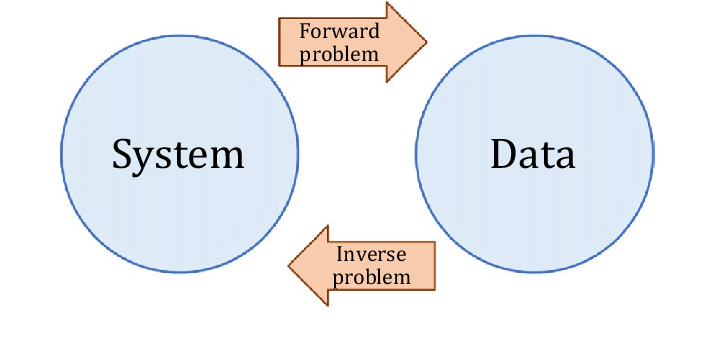
\includegraphics[width=10cm]{figs/intro/inverse_problems.png}
    \caption[Illustration of problem inversion]{Illustration of problem inversion \cite{sadri_effect_2019}}
    \label{fig:probleminv}
\end{figure}
In the context of tomography, packet level information is observe at monitors and underlying network parameters are calculated, or rather estimated in the case of stochastic tomography. Application of network tomography in this manner enables system administrators to monitor for nefarious routers with less traffic overhead and system modification compared to more conventional methods. As noted in \cref{sec:Imotivationandoutline} we aim specifically to infer the presence and location of nefariously delaying routers within the network via observations of packet delay. We expect nefarious nodes to have a more varied and heavier tailed delay distribution due to it's additional delaying of packets. To demonstrate the intuition behind this logic we provide an example firstly using path level metrics in \cref{ssec:Iex4router} then decomposing this later into router level metrics in \cref{sec:Iinferentialtechniques}.\par
In efforts to optimize stochastic network tomography we must consider how to maximise the accuracy of our analysis given the random nature of the network. Intuitively the accuracy of our analysis is limited by the amount of information we are able to collate from our probing, we employ the concept of Fisher information from the field of statistical signal detection (\cite{poor_introduction_1994}) to represent our knowledge of a single element of the network. It follows that the garnered information of all elements in the network can be presented in a Fisher information matrix (FIM) to concretely represent our knowledge of all network elements. As we are primarily measuring the variation of packet delays within the network the FIM in this context represents the information we have about queuing delays of individual routers within the network given the paths we have designed probes to take through the network.\par
In addition to quantifying our knowledge of a network the FIM has a second very desirable property of being able to quantify the minimum accuracy of estimations made about the system which it represents. This lower bound on the accuracy of inferential estimations is known as the Cramér–Rao bound (CRB) and can be seen more intuitively as the worst possible guess we can make about router's queuing delays given the probing measurements we have collected. In \cref{sec:Bparameterestimation} we cover the formal definitions and intuition behind FIM's and their corresponding CRB, later showing in \cref{sec:Mnetworkprobing} how these concepts are realised in the context of tomography. We extend on the formal definitions in \cref{sec:Boptimization} to show how the CRB, and therefore the worst possible accuracy of our guess, can be improved using an iterative approach to probe path selection. Finally after a sufficiently optimised probe path design has been determined we tackle the problem of allocation of probes between these paths. To accomplish this, techniques of optimal experiment design \cite{anthony_c_optimum_1996} are introduced in \cref{sec:Boptimization} and later used in allocation of probes to paths to maximise inferential accuracy in \cref{sec:Mnetworkprobing}.\par

\section{New Inferential Techniques}
\label{sec:Iinferentialtechniques}

Once packets are collected at each monitor node within the network the distribution of their delays is compared to that expected under different subsets of nefarious routers. The calculation of packet delays is trivial as packets traverse between monitors we are aware of both the time they are sent and the time they arrive. As the path each packet takes through the network is unknown and uncontrollable due to UR the only method of drawing inference is comparison of the observed delay distribution to what we would expect to observe assuming all possible subsets of routers are nefarious. Formally, given a network \gls{network} and set of nefarious routers \gls{nefrouters} we generate $D_G(R_N)$ where $D_x(y)$is a function computing the expected distribution vector of packet delays over a network $x$ given the set of nefarious routers $y$.\par
The computation of an expected delay vector is however non-trivial as even its approximation is dependent on \gls{qlen}, the number of time steps and the topology of \gls{network}. As presented in \cref{ssec:Icurrentmodels}, a solution in (\cite{barnes_stochastic_2020}) uses an agent based method to analytically compute the queue lengths at each router and obtain an estimation of the delay vector under the assumption that the network topology is known a priori and iterated for enough time steps to ensure it has reached a steady state. The resulting delay distribution is then compared to the observed delay distribution using techniques from signal analysis presented by \cite{lynn_introduction_2016} to obtain a correlation metric $C$ where $C(D_x,D_y)=0$ if $D_x$ has an identical distribution to $D_y$ when both distributions are probability density functions (PDFs) normalised via L2 normalization to yield the Euclidean norm. As this correlation is the only method used to gain inference, this tomographic approach is only able identify nefarious nodes within a network; sacrificing generality to any other tomographic approach as calculation of all candidate PDFs for every possible link delay or drop configuration to infer the link delay or drop metrics would be prohibitively expensive.\par
The agent based model used to generate these ‘candidate’ PDFs was produced under the same assumptions as the network tomographic model. As we are relaxing some of the tomographic models assumptions we anticipate that this agent based generation model will be insufficient to determine the nefarious router configuration resulting in the observed delay distributions. We therefore aim to establish the use of routing techniques other than UR along with new inference techniques of PDV tomography to optimize identification of nefarious routers.

\subsection{Simple PDV Tomography Example}
\label{ssec:Iex4router}
\lfix{Feel like this should be moved to methodology?}
Consider a network with 4 routers connected in a ring topology, with monitored switches at routers 0 and 3 as shown in \cref{fig:4routereg}.

\begin{figure}[H]
    \centering
    \tikzsetnextfilename{4routertopology}
    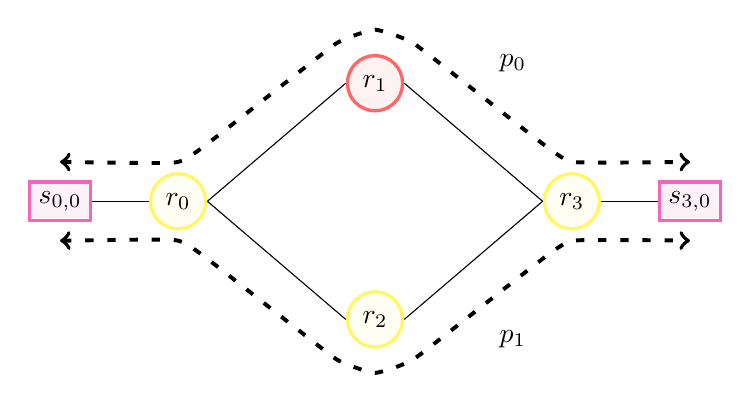
\begin{tikzpicture}[
        router/.style={circle, draw=yellow!60, fill=yellow!5, very thick, minimum size=3.5mm},
        nef_router/.style={circle, draw=red!60, fill=red!5, very thick, minimum size=3.5mm},
        switch/.style={rectangle, draw=cyan!60, fill=cyan!5, very thick, minimum size=2.5mm},
        monitor/.style={rectangle, draw=magenta!60, fill=magenta!5, very thick, minimum size=2.5mm},]
        
        % Routers
        \node[router] (r0) at (-2.5,0) {$r_0$};
        \node[nef_router] (r1) at (0,1.5)  {$r_1$};
        \node[router] (r2) at (0,-1.5) {$r_2$};
        \node[router] (r3) at (2.5,0)  {$r_3$};

        %Switches
        \node[monitor](s00) at (-4,0)   {$s_{0,0}$};
        \node[monitor] (s30) at (4,0)   {$s_{3,0}$};

        %Links
        \draw[-] (r0.east) -- (r1.west);
        \draw[-] (r0.east) -- (r2.west);
        \draw[-] (r1.east) -- (r3.west);
        \draw[-] (r2.east) -- (r3.west);
        \draw[-] (r0.west) -- (s00.east);
        \draw[-] (r3.east) -- (s30.west);
        
        % Probe path visualizations.
        \node at (1.75,1.75) {$p_0$};
        \draw[dash pattern=on 3pt off 5pt, line width=.5mm, <->] plot[smooth, tension=.2] coordinates{(-4,0.5) (-2.5,0.5) (-2,0.83) (-0.5,2) (0,2.18) (0.5,2) (2,0.83) (2.5,0.5) (4, 0.5)};
        \node at (1.75,-1.75) {$p_1$};
        \draw[dash pattern=on 3pt off 5pt, line width=.5mm, <->] plot[smooth, tension=.2] coordinates{(-4,-0.5) (-2.5,-0.5) (-2,-0.83) (-0.5,-2) (0,-2.18) (0.5,-2) (2,-0.83) (2.5,-0.5) (4,-0.5)};
    \end{tikzpicture}
    \caption{Example 4 router network.}
    \label{fig:4routereg}
\end{figure}

Let $r_1$ be a nefarious router with a $20\%$ chance of a delaying a packet at any time step. From \ref{fig:4routereg} we can see that from $s_{0,0}$ to $s_{3,0}$ there are two possible paths a packet may take: $r_0\rightarrow r_1\rightarrow r_3$ and $r_0\rightarrow r_2\rightarrow r_3$, let these paths be $p_0$ and $p_1$ respectively. Suppose we send 2,000 probe packets between $s_{0,0}$ and $s_{3,0}$, let $\phi_0$ and $\phi_1$ be the probability of a packet being sent along $p_0$ or $p_1$ respectively.\par
At the end of the measurement interval, the difference in time from each packet being sent from $s_{0,0}$ and the received by $s_{3,0}$ is recorded to calculate the delay of each packet. Ignoring background traffic for illustrative proposes we obtain the delay histograms shown in \cref{fig:ppdelayhist}. Visually we can confirm our expectation of the path with the delaying router $r_1$ having a heavier tailed distribution.\par
\begin{figure}[H]
    \begin{subfigure}[b]{0.475\textwidth}
        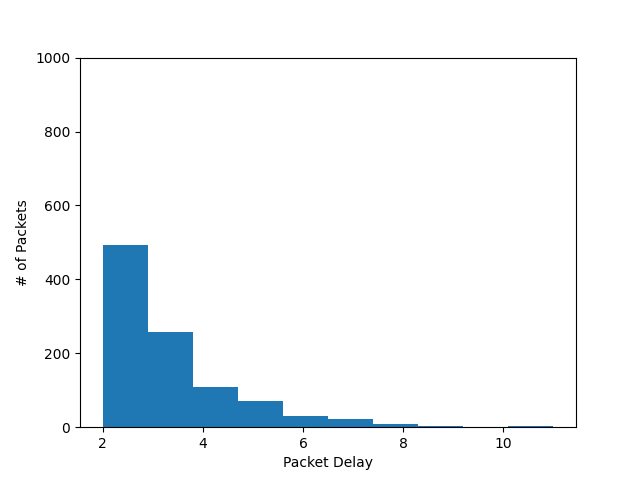
\includegraphics[width=\textwidth]{figs/intro/p0_delayhist.png}
        \caption[]{Delays over $p_0$.}
    \end{subfigure}
    \begin{subfigure}[b]{0.475\textwidth}
        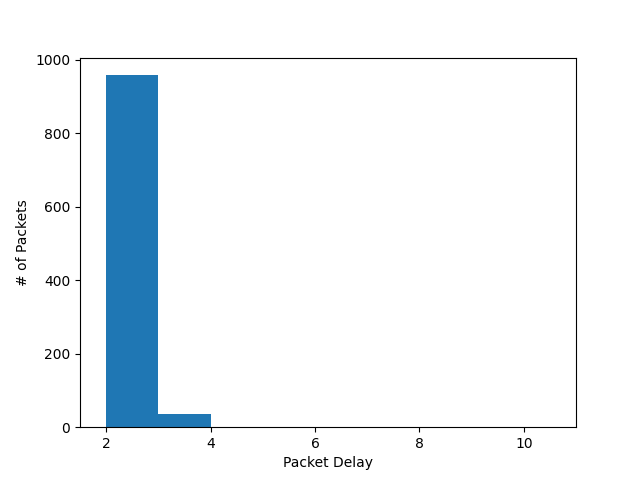
\includegraphics[width=\textwidth]{figs/intro/p1_delayhist.png}
        \caption[]{Delays over $p_1$.}
    \end{subfigure}
    \caption{Histograms of probe path level delays for a 4 router ring network.}
    \label{fig:ppdelayhist}
\end{figure}
From these distributions we compute the mean and delay variance for each path, obtaining values in \cref{tbl:4routerstats}. In this analytical approach the correlation between nefarious router behaviour and path level packet delay becomes glaringly obvious with an almost 200\% increase of delay variance in the path $p_0$ containing the nefarious router $r_1$. Probe path level analysis as we have conducted here however is not sufficient to enable distinction of all routers within a network. Even in this minimal example we have explored, $r_0$ and $r_3$ exists on both $p_0$ and $p_1$, if either router was nefarious it would impact both path measurements equally and as such be undetectable. To resolve this problem we extend this method with node identification techniques in \cref{sec:Mnetworkprobing} to enable computation of router level packet delay statistics in \cref{sec:Maddtomography} .
\begin{table}[H]
    \centering
    \begin{tabular}{@{}ccc@{}}
        \toprule
        & \multicolumn{2}{c}{\textbf{Probe path}}\\
        \cmidrule(lr){2-3}
        Measure & $p_0$ & $p_1$ \\
        \midrule
        $\bar{x}$   & 3.03 & 2.04 \\
        $\sigma$    & 1.42 & 0.19 \\
        $\sigma^2$  & 2.03 & 0.03 \\
        \bottomrule
    \end{tabular}
    \caption{Measures of center and spread for packet delays in a 4 router network.}
    \label{tbl:4routerstats}
\end{table}

\section{Summary}
\label{sec:Iintroductionsummary}

In this section we have expanded upon the problem of improving existing simulations. We note it serves to treat it instead as 3 separate but related problems of optimisations and extension at each of the previously listed stages. This is as the work done at each stage can be entirely self contained and parsed to another if required, the network can be generated at at earlier point in time, stored and later given to the network traffic simulation, likewise the metrics measures from this simulation can be stored and later used to calculate probabilities of a given router being nefarious.\par
Optimisation to the code for time complexity is desirable as it allows for larger simulations to be run for more time steps given limited compute resources available. Such extended run time allow for statistical approximations to converge as seen in \cref{cha:result}. The simulation of larger networks also allows for the inclusion of real world network topologies such as \cite{cadi_caida_2002}, \cite{university_of_washington_rocketfuel_2002}, \cite{medina_brite_2001} for analysis, a key requirement for the goal of this body of work. The final artifact of code is presented and made available at (\cite{sylvester_millar_real_2021}) in hopes that future work will be able to use this to further expand on this area of work, specific extensions are highlighted in \cref{cha:conc}.